\section{Definição}

\begin{frame}[fragile]{{\it Definição}}

    \metroset{block=fill}
    \begin{block}{Problema do Troco}
        Seja $C = \{c_1, c_2, \ldots, c_N\}$ uma sequência ordenada de $N$ inteiros positivos
        distintos
        e $M$ um inteiro positivo. O problema do troco consiste em determinar um vetor de inteiros
        não-negativos $x = \{ x_1, x_2, \ldots, x_N \}$ tal que
        \[
            M = \sum_{i = 1}^N x_ic_i
        \]
        e que a soma
        \[
            S = \sum_{i = 1}^N x_i
        \] seja mínima.
    \end{block}

\end{frame}

\begin{frame}[fragile]{Características do problema do troco}

    \begin{itemize}
        \item Os elementos do conjunto $C$ são denominados \textit{moedas}

        \item $M$ é o \textit{troco}

        \item O problema pode ser definido informalmente como: \textit{Qual é o menor número de
            moedas necessárias para dar o troco $M$?}

        \item Se $c_1 = 1$, há solução para qualquer $M$

        \item Se $C$ é o conjunto de moedas utilizadas no sistema financeiro da maioria dos
            países, o problema do troco pode ser resolvido por meio de um algoritmo guloso
    \end{itemize}

\end{frame}

\begin{frame}[fragile]{Algoritmo guloso para o problema do troco}

    \begin{itemize}
        \item O algoritmo guloso para o problema do troco escolhe, dentre as moedas, a maior delas
            que é menor ou igual a $M$ (assuma que esta seja a moeda $c_k$)

        \item Em seguida, ele atribui a $x_k$ o valor $M/c_k$ e subtrai de $M$ o valor $x_kc_k$

        \item O algoritmo então prossegue até que $M$ se torne igual a zero
            
        \item Para todos os valores $x_i$ não atribuídos durante o algoritmo, vale que $x_i = 0$ 

    \end{itemize}

\end{frame}

\begin{frame}[fragile]{Visualização do algoritmo guloso para o problema do troco}

    \begin{figure}
        \centering

        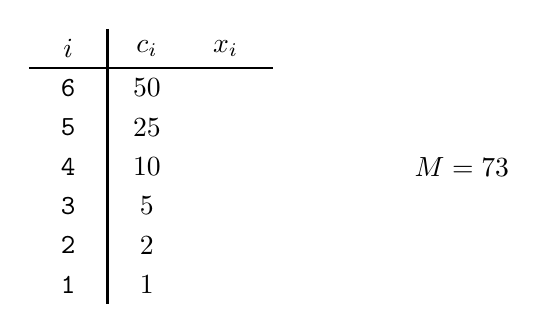
\begin{tikzpicture}
            \node at (5, 4) { $M = 73$ };

            \draw[thick] (-0.5, 5.25) -- (2.6, 5.25);
            \draw[thick] (0.5, 5.75) -- (0.5, 2.25);

            \node at (0, 5.5) { $i$ };
            \node at (0, 5) { \tt 6 };
            \node at (0, 4.5) { \tt 5 };
            \node at (0, 4) { \tt 4 };
            \node at (0, 3.5) { \tt 3 };
            \node at (0, 3) { \tt 2 };
            \node at (0, 2.5) { \tt 1 };

            \node at (1, 5.5) { $c_i$ };
            \node at (1, 5) { $50$ };
            \node at (1, 4.5) { $25$ };
            \node at (1, 4) { $10$ };
            \node at (1, 3.5) { $5$ };
            \node at (1, 3) { $2$ };
            \node at (1, 2.5) { $1$ };

            \node at (2, 5.5) { $x_i$ };
            %\node at (2, 5) { $50$ };
            %\node at (2, 4.5) { $25$ };
            %\node at (2, 4) { $10$ };
            %\node at (2, 3.5) { $5$ };
            %\node at (2, 3) { $2$ };
            %\node at (2, 2.5) { $1$ };


        \end{tikzpicture}

    \end{figure}

\end{frame}

\begin{frame}[fragile]{Visualização do algoritmo guloso para o problema do troco}

    \begin{figure}
        \centering

        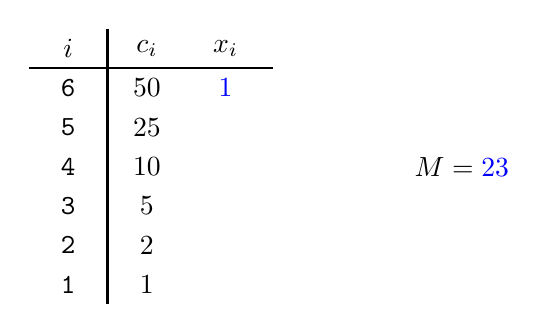
\begin{tikzpicture}
            \node at (5, 4) { $M = \textcolor{blue}{23}$ };

            \draw[thick] (-0.5, 5.25) -- (2.6, 5.25);
            \draw[thick] (0.5, 5.75) -- (0.5, 2.25);

            \node at (0, 5.5) { $i$ };
            \node at (0, 5) { \tt 6 };
            \node at (0, 4.5) { \tt 5 };
            \node at (0, 4) { \tt 4 };
            \node at (0, 3.5) { \tt 3 };
            \node at (0, 3) { \tt 2 };
            \node at (0, 2.5) { \tt 1 };

            \node at (1, 5.5) { $c_i$ };
            \node at (1, 5) { $50$ };
            \node at (1, 4.5) { $25$ };
            \node at (1, 4) { $10$ };
            \node at (1, 3.5) { $5$ };
            \node at (1, 3) { $2$ };
            \node at (1, 2.5) { $1$ };

            \node at (2, 5.5) { $x_i$ };
            \node at (2, 5) { \textcolor{blue}{$1$} };
            %\node at (2, 4.5) { $25$ };
            %\node at (2, 4) { $10$ };
            %\node at (2, 3.5) { $5$ };
            %\node at (2, 3) { $2$ };
            %\node at (2, 2.5) { $1$ };


        \end{tikzpicture}

    \end{figure}

\end{frame}

\begin{frame}[fragile]{Visualização do algoritmo guloso para o problema do troco}

    \begin{figure}
        \centering

        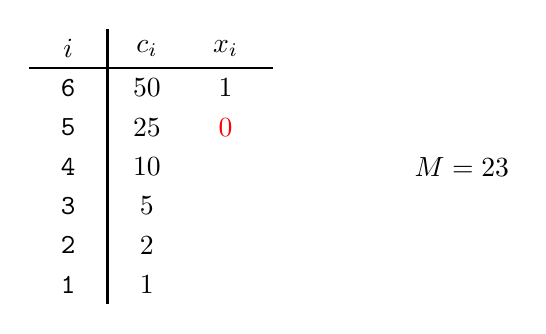
\begin{tikzpicture}
            \node at (5, 4) { $M = \textcolor{black}{23}$ };

            \draw[thick] (-0.5, 5.25) -- (2.6, 5.25);
            \draw[thick] (0.5, 5.75) -- (0.5, 2.25);

            \node at (0, 5.5) { $i$ };
            \node at (0, 5) { \tt 6 };
            \node at (0, 4.5) { \tt 5 };
            \node at (0, 4) { \tt 4 };
            \node at (0, 3.5) { \tt 3 };
            \node at (0, 3) { \tt 2 };
            \node at (0, 2.5) { \tt 1 };

            \node at (1, 5.5) { $c_i$ };
            \node at (1, 5) { $50$ };
            \node at (1, 4.5) { $25$ };
            \node at (1, 4) { $10$ };
            \node at (1, 3.5) { $5$ };
            \node at (1, 3) { $2$ };
            \node at (1, 2.5) { $1$ };

            \node at (2, 5.5) { $x_i$ };
            \node at (2, 5) { \textcolor{black}{$1$} };
            \node at (2, 4.5) { \textcolor{red}{$0$} };
            %\node at (2, 4) { $10$ };
            %\node at (2, 3.5) { $5$ };
            %\node at (2, 3) { $2$ };
            %\node at (2, 2.5) { $1$ };


        \end{tikzpicture}

    \end{figure}

\end{frame}

\begin{frame}[fragile]{Visualização do algoritmo guloso para o problema do troco}

    \begin{figure}
        \centering

        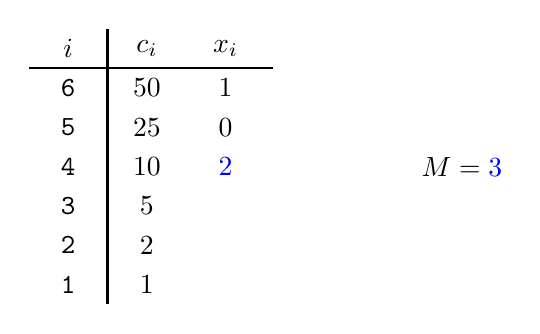
\begin{tikzpicture}
            \node at (5, 4) { $M = \textcolor{blue}{3}$ };

            \draw[thick] (-0.5, 5.25) -- (2.6, 5.25);
            \draw[thick] (0.5, 5.75) -- (0.5, 2.25);

            \node at (0, 5.5) { $i$ };
            \node at (0, 5) { \tt 6 };
            \node at (0, 4.5) { \tt 5 };
            \node at (0, 4) { \tt 4 };
            \node at (0, 3.5) { \tt 3 };
            \node at (0, 3) { \tt 2 };
            \node at (0, 2.5) { \tt 1 };

            \node at (1, 5.5) { $c_i$ };
            \node at (1, 5) { $50$ };
            \node at (1, 4.5) { $25$ };
            \node at (1, 4) { $10$ };
            \node at (1, 3.5) { $5$ };
            \node at (1, 3) { $2$ };
            \node at (1, 2.5) { $1$ };

            \node at (2, 5.5) { $x_i$ };
            \node at (2, 5) { \textcolor{black}{$1$} };
            \node at (2, 4.5) { \textcolor{black}{$0$} };
            \node at (2, 4) { \textcolor{blue}{$2$} };
            %\node at (2, 3.5) { $5$ };
            %\node at (2, 3) { $2$ };
            %\node at (2, 2.5) { $1$ };


        \end{tikzpicture}

    \end{figure}

\end{frame}

\begin{frame}[fragile]{Visualização do algoritmo guloso para o problema do troco}

    \begin{figure}
        \centering

        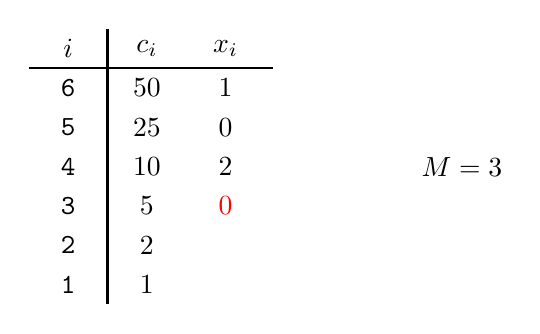
\begin{tikzpicture}
            \node at (5, 4) { $M = \textcolor{black}{3}$ };

            \draw[thick] (-0.5, 5.25) -- (2.6, 5.25);
            \draw[thick] (0.5, 5.75) -- (0.5, 2.25);

            \node at (0, 5.5) { $i$ };
            \node at (0, 5) { \tt 6 };
            \node at (0, 4.5) { \tt 5 };
            \node at (0, 4) { \tt 4 };
            \node at (0, 3.5) { \tt 3 };
            \node at (0, 3) { \tt 2 };
            \node at (0, 2.5) { \tt 1 };

            \node at (1, 5.5) { $c_i$ };
            \node at (1, 5) { $50$ };
            \node at (1, 4.5) { $25$ };
            \node at (1, 4) { $10$ };
            \node at (1, 3.5) { $5$ };
            \node at (1, 3) { $2$ };
            \node at (1, 2.5) { $1$ };

            \node at (2, 5.5) { $x_i$ };
            \node at (2, 5) { \textcolor{black}{$1$} };
            \node at (2, 4.5) { \textcolor{black}{$0$} };
            \node at (2, 4) { \textcolor{black}{$2$} };
            \node at (2, 3.5) { \textcolor{red}{$0$} };
            %\node at (2, 3) { $2$ };
            %\node at (2, 2.5) { $1$ };


        \end{tikzpicture}

    \end{figure}

\end{frame}

\begin{frame}[fragile]{Visualização do algoritmo guloso para o problema do troco}

    \begin{figure}
        \centering

        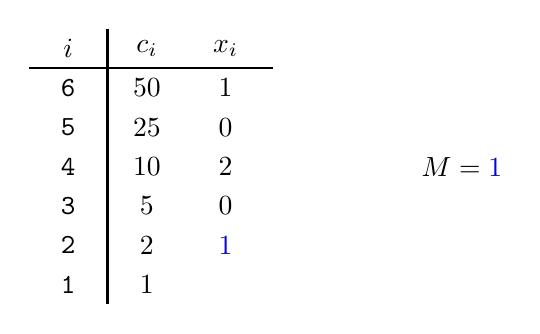
\begin{tikzpicture}
            \node at (5, 4) { $M = \textcolor{blue}{1}$ };

            \draw[thick] (-0.5, 5.25) -- (2.6, 5.25);
            \draw[thick] (0.5, 5.75) -- (0.5, 2.25);

            \node at (0, 5.5) { $i$ };
            \node at (0, 5) { \tt 6 };
            \node at (0, 4.5) { \tt 5 };
            \node at (0, 4) { \tt 4 };
            \node at (0, 3.5) { \tt 3 };
            \node at (0, 3) { \tt 2 };
            \node at (0, 2.5) { \tt 1 };

            \node at (1, 5.5) { $c_i$ };
            \node at (1, 5) { $50$ };
            \node at (1, 4.5) { $25$ };
            \node at (1, 4) { $10$ };
            \node at (1, 3.5) { $5$ };
            \node at (1, 3) { $2$ };
            \node at (1, 2.5) { $1$ };

            \node at (2, 5.5) { $x_i$ };
            \node at (2, 5) { \textcolor{black}{$1$} };
            \node at (2, 4.5) { \textcolor{black}{$0$} };
            \node at (2, 4) { \textcolor{black}{$2$} };
            \node at (2, 3.5) { \textcolor{black}{$0$} };
            \node at (2, 3) { \textcolor{blue}{$1$} };
            %\node at (2, 2.5) { $1$ };


        \end{tikzpicture}

    \end{figure}

\end{frame}

\begin{frame}[fragile]{Visualização do algoritmo guloso para o problema do troco}

    \begin{figure}
        \centering

        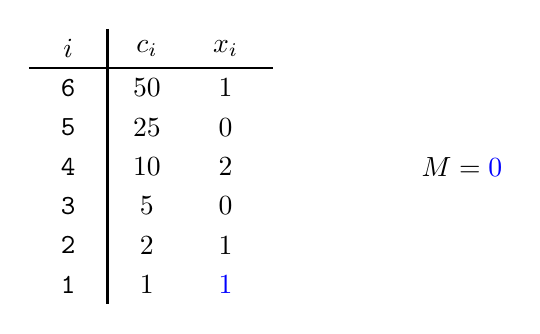
\begin{tikzpicture}
            \node at (5, 4) { $M = \textcolor{blue}{0}$ };

            \draw[thick] (-0.5, 5.25) -- (2.6, 5.25);
            \draw[thick] (0.5, 5.75) -- (0.5, 2.25);

            \node at (0, 5.5) { $i$ };
            \node at (0, 5) { \tt 6 };
            \node at (0, 4.5) { \tt 5 };
            \node at (0, 4) { \tt 4 };
            \node at (0, 3.5) { \tt 3 };
            \node at (0, 3) { \tt 2 };
            \node at (0, 2.5) { \tt 1 };

            \node at (1, 5.5) { $c_i$ };
            \node at (1, 5) { $50$ };
            \node at (1, 4.5) { $25$ };
            \node at (1, 4) { $10$ };
            \node at (1, 3.5) { $5$ };
            \node at (1, 3) { $2$ };
            \node at (1, 2.5) { $1$ };

            \node at (2, 5.5) { $x_i$ };
            \node at (2, 5) { \textcolor{black}{$1$} };
            \node at (2, 4.5) { \textcolor{black}{$0$} };
            \node at (2, 4) { \textcolor{black}{$2$} };
            \node at (2, 3.5) { \textcolor{black}{$0$} };
            \node at (2, 3) { \textcolor{black}{$1$} };
            \node at (2, 2.5) { \textcolor{blue}{$1$} };


        \end{tikzpicture}

    \end{figure}

\end{frame}


\begin{frame}[fragile]{Implementação do algoritmo guloso para o problema do troco}
    \inputsnippet{cpp}{1}{17}{codes/greedy.cpp}
\end{frame}

\begin{frame}[fragile]{Implementação do algoritmo guloso para o problema do troco}
    \inputsnippet{cpp}{19}{39}{codes/greedy.cpp}
\end{frame}

\begin{frame}[fragile]{Incorretude do algoritmo guloso}

    \begin{itemize}
        \item O algoritmo guloso para o problema do troco, porém, não produz a solução correta para
            todas as entradas possíveis

        \item Por exemplo, se $C = \{ 1, 4, 5 \}$ e $M = 8$, o algoritmo guloso retornaria 4
            moedas: uma de 5 e três de 1

        \item Contudo, é possível dar um troco de 8 com apenas duas moedas de 4

        \item Assim, para obter a solução correta para qualquer troco e qualquer conjunto de 
            moedas, é preciso utilizar um algoritmo baseado em outro paradigma que não o guloso
            
    \end{itemize}

\end{frame}

\begin{frame}[fragile]{Algoritmo de programação dinâmica}

    \begin{itemize}
        \item A programação dinâmica pode ser utilizada para desenvolver um algoritmo correto para
            o problema do troco

        \item Seja $c(m)$ o mínimo de moedas necessárias para um troco igual a $m$

        \item O caso base acontece quando $m = 0$: neste caso, $c(0) = 0$

        \item As transições acontecem para cada uma das moedas $c_k \leq m$:
        \[
            c(m) = \min\{ c(m - c_{k_1}), c(m - c_{k_2}), \ldots, c(m - c_{k_r}) \} + 1
        \]

        \item Isto corresponde a escolher uma moeda (o termo +1) que seja menor ou igual ao troco e
            computar o troco mínimo para o restante

        \item São $O(M)$ estados distintos e as transições são feitas em $O(N)$

        \item Portanto a complexidade do algoritmo é $O(MN)$
    \end{itemize}

\end{frame}

\begin{frame}[fragile]{Algoritmo de programação dinâmica para o problema do troco}
    \inputsnippet{cpp}{1}{20}{codes/cc.cpp}
\end{frame}

\begin{frame}[fragile]{Algoritmo de programação dinâmica para o problema do troco}
    \inputsnippet{cpp}{22}{42}{codes/cc.cpp}
\end{frame}

\begin{frame}[fragile]{Implementação {\it bottom-up}}

    \begin{itemize}
        \item O estado e as transições apresentadas anteriormente permite uma implementação
            \textit{bottom-up} do algoritmo de programação dinâmica para o problema do troco

        \item O natural seria um laço externo, com o troco $m$ variando de $0$ a $M$, e um laço
            interno, avaliando as $N$ moedas

        \item Embora a complexidade permaneça a mesma da implementação \textit{top-down}, esta
            ordem não é favorável à \textit{cache}, por conta dos diferentes saltos associados
            às moedas

        \item É possível melhorar a performance em tempo de execução invertendo os laços: para
            cada moeda, deve-se avaliar todos os trocos possíveis
    \end{itemize}

\end{frame}

\begin{frame}[fragile]{Implementação {\it bottom-up} para o problema do troco}
    \inputsnippet{cpp}{1}{20}{codes/cc_bu.cpp}
\end{frame}

\begin{frame}[fragile]{Implementação {\it bottom-up} para o problema do troco}
    \inputsnippet{cpp}{22}{42}{codes/cc_bu.cpp}
\end{frame}




